\section{Noise Description}

As mentioned in~\cite{Yahia2013}, there are four main noise sources in the receiver.
In the following each noise source will be described and its transfer function towards the loads will be derived. 

\subsection{Antenna Noise}
\label{sec:antenna_noise}

The antennas introduce two noise sources.
The external noise $\vec{n}_{ext}$, collected from the radiation component of the antenna array and the noise generated by the losses in the antennas $\vec{n}_l$.
From~\cite{Twiss1955} it follows, 
\begin{equation}
\label{eq:cov_ant}
\mat{R}_{na} = \mathbb{E}[\vec{n}_{AR}\vec{n}_{AR}^H] = 4 k_B B_W(T_{AE}\mathbb{R}\{\mat{Z}_{AR}\}+T_{AL}\mat{R}_{AR}),
\end{equation}
with $k_B$ the Boltzmann constant and $B_W$ the bandwidth.

\subsubsection{Transfer Function of the Antenna Noise}
\label{sec:antenna_noise_transf}
As the antenna noise is picked up by the antennas in the same way as the signal, the transfer function remains the same as the one derived in Section~\ref{sec:transf} for the signal, e.g.
\begin{align}
\mat{H}_{L,0} &= \mat{H}_{L,LNA}\cdot\mat{H}_{LNA,M}\cdot\mat{H}_{M,0},\quad\text{including port reduction}\\\nonumber
\mat{H}_{L,0} &= \mat{H}_{L,LNA}\cdot\mat{H}_{LNA,M}\cdot\mat{H}_{M,0}\cdot\mat{H}_{0}.
\end{align}

\subsection{LNA Noise}
\label{sec:lna_noise}

The LNA introduces the third noise source.
From the discussion in~\cite{Nossek}, the noise of the LNA is modeled by a series of voltages and parallel currents at the input of the LNA.
The noise sources have the following statistical properties,
\begin{align}
\label{eq:cov_lna}
\mathbb{E}[\vec{i}_{LNA}\vec{i}_{LNA}^H] &= \beta \mat{I}_{N_r},\\\nonumber
\mathbb{E}[\vec{v}_{LNA}\vec{v}_{LNA}^H] &= \beta R_n^2\mat{I}_{N_r},\quad\text{and}\\\nonumber
\mathbb{E}[\vec{v}_{LNA}\vec{i}_{LNA}^H] &= \rho \beta R_n\mat{I}_{N_r},
\end{align}
with $\rho$ and $\beta$ as correlation coefficients.

\subsubsection{Transfer Function of the LNA Noise}
\label{sec:antenna_noise_transf}
As written above, we have two noise sources, the serial voltage sources and the parallel current sources.
First we will transfer the current source into a voltage source in series as we then can use the same transfer function for the voltage and the transferred current sources.
To do so, we need the equivalent input impedances looking from the left into the LNA block and from the right into the matching network.
The equivalent input impedance for the LNA network $\mat{Z}_{eqLNA_1}$ was already derived in~\eqref{eq:zeqlna1}.
To get the equivalent input impedance for the matching network looking from the right into it we use Equation~\eqref{eq:eq_imp_load} and get
\begin{align}
\label{eq:zr}
\mat{\tilde{Z}}_{eqM_2} &= \mat{Z}_{M22} - \mat{Z}_{M12}\cdot(\mat{Z}_{M11} + \mat{Z}_{C'})^{-1}\cdot\mat{Z}_{M21}.
\end{align}

Transferring the current source into a series of voltages gives us 
\begin{equation}
\vec{v}_{LNA_c} = -\mat{\tilde{Z}}_{eqM_2} \vec{i}_{LNA},
\end{equation}

and therefore a transfer function of
\begin{equation}
\mat{H}_{L,LNA_v} = R_L\mat{I}_{N_r}(R_L\mat{I}_{N_r} + \mat{\tilde{Z}}_{eqLNA_2})^{-1}\mat{e}\cdot(\mat{c}+\mat{\tilde{Z}}_{eqM_2})^{-1},
\end{equation}
for the series voltages and
\begin{equation}
\mat{H}_{L,LNA_c} = -R_L\mat{I}_{N_r}(R_L\mat{I}_{N_r} + \mat{\tilde{Z}}_{eqLNA_2})^{-1}\mat{e}\cdot(\mat{c}+\mat{\tilde{Z}}_{eqM_2})^{-1}\mat{\tilde{Z}}_{eqM_2},
\end{equation}
for the LNA noise currents.



\subsection{Downstream Noise}
\label{sec:down_noise}
The last noise source is the downstream noise, generated by all the circuitry after the LNA~\cite{Hughes2012} and modeled by voltage sources $\vec{\tilde{v}}_n$ in series to the loads.
With the statistical property
\begin{equation}
\label{eq:cov_down}
\mathbb{E}[\vec{\tilde{v}}_n\vec{\tilde{v}}_n^H] = \psi\mat{I}_{N_r}.
\end{equation}

\subsubsection{Transfer Function of the Downstream Noise}
\label{sec:down_noise_transf}
For the transfer function of the downstream noise we need a simple voltage divider of the loads and the equivalent input impedance $\mat{\tilde{Z}}_{eqLNA_2}$ looking from the right into the LNA block.
Note, that this is NOT the same input impedance as in~\eqref{eq:zeqlna2}.
Therefore the transfer function becomes
\begin{equation}
\mat{H}_{L,n} = R_L\mat{I}_{N_r}(R_L\mat{I}_{N_r} + \mat{\tilde{Z}}_{eqLNA_2})^{-1},
\end{equation}
with 
\begin{align}
\label{eq:zeqlna2_down}
\mat{\tilde{Z}}_{eqLNA_2} &= \mat{g} - \mat{d}\cdot(\mat{c} + \mat{\tilde{Z}}_{eqM_2})^{-1}\cdot\mat{e} = \mat{g}.
\end{align}
However, under the unilateral assumption the input impedance reduces to $\mat{\tilde{Z}}_{eqLNA_2} = \mat{g}$.


\subsection{Noise Coupling}
\label{sec:noise_coupling}

So far we transferred the noise from it's source to the loads behind the LNA block.
However additionally to the direct path, we need to take the noise of different receiver branches into account.
Therefore we transfer the noise sources to series voltages next to the antenna voltages, so that we can use the transfer functions derived in Chapter~\ref{sec:network_description}.

As in the previous Section, we consider again the four noise types.
For the antenna noise, we note, that we do not need to derive a transfer function.
In a first step we transfer the LNA-current noise source and the downstream noise to the LNA-voltage noise source.
Therefore the LNA-current noise source is multiplied by the equivalent input impedance of the LNA
\begin{align}
\vec{v}_{LNAc} = \mat{Z}_{eqLNA_1} \vec{i}_{LNA}.
\end{align}
For the downstream noise we note, that under the unilateral assumption, the transferred noise is zero, else
\begin{align}
\vec{v}_{LNAn} = \mat{d}(\mat{g}+R_L\mat{I}_{N_R})^{-1} \tilde{\vec{v}}_{v}.
\end{align}

Now we only need to find the transfer function for the LNA-voltage source $\vec{v}_{LNAv}$.
The transfer function over the matching network is given by
\begin{align}
\label{eq:noise_to_input}
\mat{H}_{0,LNA} = \mat{Z}_{M12}(\mat{Z}_{M22}+\mat{Z}_{eqLNA_1})^{-1}.
\end{align}




\subsection{Noise Covariance Matrix}
\label{sec:sig_cov}

\begin{figure}[h]
\begin{center}
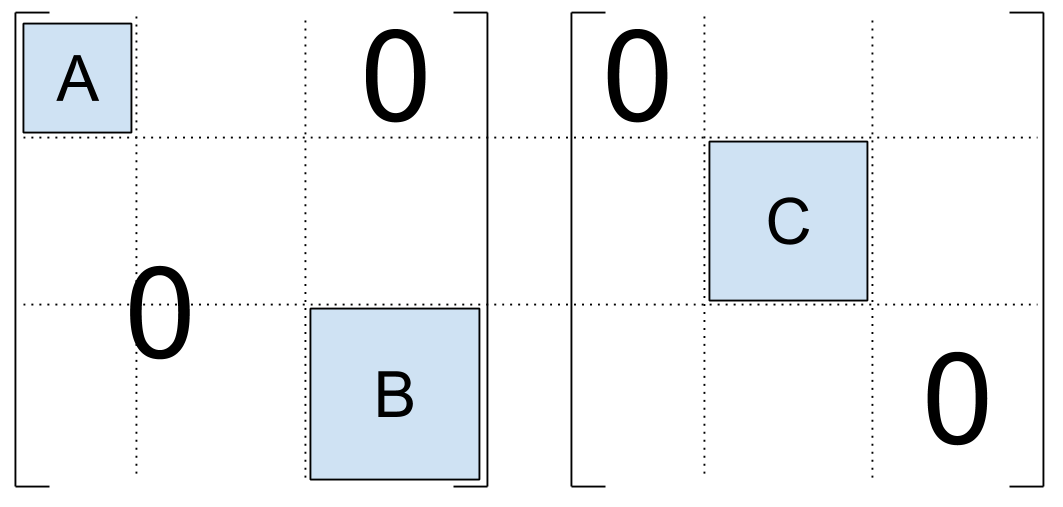
\includegraphics[width=0.75\textwidth]{images/matrix_shaping.png}
\caption{An example of the matrix shaping function. On the left the matrix shaped by $\Gamma(\cdot)$ on the right the matrix shaped by $\Gamma(\cdot)^{-1}$. The sub matrices $\mat{A},\mat{B}$ and $\mat{C}$ are square matrices and lie on the diagonal.}
\label{fig:matrix_shaping}
\end{center}
\end{figure}

As in Chapter~\ref{sec:network_description}, we will derive the noise covariance matrix.
To do so, we introduce the function $\Gamma(\cdot)$, which reshapes the matrices to our needs.
For example Equation~\eqref{eq:noise_to_input} must only be applied on the noise sources of the receivers, which shall be reduced, however a multiplication of the transfer matrix with the full noise vector is desired.
Let further $\Gamma(\cdot)^{-1}$, denote the function, which shapes the matrices only to the branches which are not reduced.
We note the following properties of the function:
\begin{align}
\label{eq:gamma_properties}\nonumber
\Gamma(\mat{A})\cdot\Gamma(\mat{B}) &= \Gamma(\mat{A}\cdot\mat{B}),\\\nonumber
\Gamma(\mat{A}^{H}) &= \Gamma(\mat{A})^{H},\\\nonumber
\Gamma(\mat{A})\cdot\Gamma(\mat{B})^{-1} &= \mat{0},\quad\text{and}\\
\forall \mat{A},\mat{B},\quad\text{which form a}&\text{ valid matrix multiplication}\quad\mat{A}\cdot\mat{B}.
\end{align}
Note that the first two properties are also valid for $\Gamma(\cdot)^{-1}$.
Additionally for diagonal matrices the following property holds $\Gamma(\mat{A})+\Gamma(\mat{A})^{-1} = \mat{A}$.

As we have multiple noise sources, first we will describe the noise output $\vec{u}_L$ for each noise source, i.e.:
\begin{align}
\label{eq:noise_output}
\nonumber
\vec{u}_{AR} &= \mat{H}_{L,0}\cdot\vec{n}_{AR},\\\nonumber 
\vec{u}_{LNA_v} &= \left(\mat{H}_{L,0}\cdot\Gamma(\mat{H}_{0,LNA})+\Gamma(\mat{H}_{L,LNA_v})^{-1}\right)\cdot\vec{v}_{LNA},\\\nonumber
\vec{u}_{LNA_c} &= \left(\mat{H}_{L,0}\cdot\Gamma(\mat{H}_{0,LNA}\mat{Z}_{eqLNA_1})+\Gamma(\mat{H}_{L,LNA_c})^{-1}\right)\cdot\vec{i}_{LNA},\\\nonumber
\vec{u}_{\tilde{n}} &= \left(\mat{H}_{L,0}\cdot\Gamma(\mat{H}_{0,LNA}\cdot\mat{d}(\mat{g}+R_L\mat{I}_{N_R})^{-1})+\Gamma(\mat{H}_{L,n})^{-1}\right)\cdot\vec{\tilde{v}}_{n},\\
\text{and therefore}\qquad &\vec{u}_L = \vec{u}_{AR} + \vec{u}_{LNA_v} + \vec{u}_{LNA_c} + \vec{u}_{\tilde{n}}.
\end{align}

Because all the noise sources are uncorrelated, except for the LNA noise sources (Equation~\eqref{eq:lna_noise}), the noice covariance matrix can be written as:
\begin{align}
\label{eq:exp_noise}\nonumber
\mat{K}_n =\mathbb{E}[\vec{u}_L\vec{u}_L^H] = &\mat{H}_{L,0}\mathbb{E}[\vec{n}_{AR}\vec{n}_{AR}^H]\mat{H}_{L,0}^H + 
\mathbb{E}[\vec{u}_{LNA_v}\vec{u}_{LNA_v}^H] +
\mathbb{E}[\vec{u}_{LNA_v}\vec{u}_{LNA_c}^H] +\\%\nonumber
\quad&\mathbb{E}[\vec{u}_{LNA_c}\vec{u}_{LNA_v}^H] +
\mathbb{E}[\vec{u}_{LNA_c}\vec{u}_{LNA_c}^H] +
\mathbb{E}[\vec{u}_{\tilde{n}}\vec{u}_{\tilde{n}}^H]
%\\\nonumber
%&\mat{H}_{L,LNA_v}\mathbb{E}[\vec{v}_{LNA}\vec{v}_{LNA}^H]\mat{H}_{L,LNA_v}^H -\\\nonumber
%&\mat{H}_{L,LNA_v}\mathbb{E}[\vec{v}_{LNA}\vec{i}_{LNA}^H]\mat{H}_{L,LNA_c}^H -
%\mat{H}_{L,LNA_c}\mathbb{E}[\vec{i}_{LNA}\vec{v}_{LNA}^H]\mat{H}_{L,LNA_v}^H + \\
%&\mat{H}_{L,LNA_c}\mathbb{E}[\vec{i}_{LNA}\vec{i}_{LNA}^H]\mat{H}_{L,LNA_c}^H +
%\mat{H}_{L,n}\mathbb{E}[\vec{\tilde{v}}_{n}\vec{\tilde{v}}_{n}^H]\mat{H}_{L,n}^H .
\end{align}

For simplicity reasons, we will look in every summand seperately in the following.
As $-\mat{H}_{L,LNA_v}\cdot\mat{\tilde{Z}}_{eqM_2} = \mat{H}_{L,LNA_c}$ and using~\eqref{eq:cov_ant},~\eqref{eq:cov_lna},~\eqref{eq:cov_down} and~\eqref{eq:gamma_properties}, it follows
\begin{align}
\nonumber
\mat{K}_{n_{LNA_{vv}}} &= \mathbb{E}\left[\left(\mat{H}_{L,0}\cdot\Gamma(\mat{H}_{0,LNA})+\Gamma(\mat{H}_{L,LNA_v})^{-1}\right)\cdot\vec{v}_{LNA}\vec{v}_{LNA}^H\cdot\right.\\\nonumber
&\qquad\left.\left(\mat{H}_{L,0}\cdot\Gamma(\mat{H}_{0,LNA})+\Gamma(\mat{H}_{L,LNA_v})^{-1}\right)^H\right]\\\nonumber
&=\left(\mat{H}_{L,0}\cdot\Gamma(\mat{H}_{0,LNA})+\Gamma(\mat{H}_{L,LNA_v})^{-1}\right)\cdot\mathbb{E}\left[\vec{v}_{LNA}\vec{v}_{LNA}^H\right]\cdot\\\nonumber
&\qquad\left(\mat{H}_{L,0}\cdot\Gamma(\mat{H}_{0,LNA})+\Gamma(\mat{H}_{L,LNA_v})^{-1}\right)^H\\
&=\beta R_n^2\left(\mat{H}_{L,0}\cdot\Gamma\left(\mat{H}_{0,LNA}\mat{H}_{0,LNA}^H\right)\mat{H}_{0,LNA}^H+\Gamma\left(\mat{H}_{L,LNA_v}\mat{H}_{L,LNA_v}^H\right)^{-1}\right),
\end{align}
for the LNA-voltage source and
\begin{align}
\nonumber
\mat{K}_{n_{LNA_{cc}}} &= 
\beta \biggl(\mat{H}_{L,0}\cdot\Gamma\left(\mat{H}_{0,LNA}\mat{Z}_{eqLNA_1}\mat{Z}_{eqLNA_1}^H\mat{H}_{0,LNA}^H\right)\mat{H}_{0,LNA}^H+\\
&\qquad\left.\Gamma\left(\mat{H}_{L,LNA_v}\mat{\tilde{Z}}_{eqM_2}\mat{\tilde{Z}}_{eqM_2}^H\mat{H}_{L,LNA_v}^H\right)^{-1}\right),
\end{align}
for the LNA-current source.
For the cross terms it follows
\begin{align}
\nonumber
\mat{K}_{n_{LNA_{vc}}} &= \rho\beta R_n
\left(\mat{H}_{L,0}\cdot\Gamma\left(\mat{H}_{0,LNA}\mat{Z}_{eqLNA_1}^H\mat{H}_{0,LNA}^H\right)\mat{H}_{L,0}^H + 
\Gamma\left(\mat{H}_{L,LNA_v}\mat{\tilde{Z}}_{eqM_2}^H\mat{H}_{L,LNA_v}^H\right)^{-1}\right)\\\nonumber
&\quad+
\rho^*\beta R_n
\left(\mat{H}_{L,0}\cdot\Gamma\left(\mat{H}_{0,LNA}\mat{Z}_{eqLNA_1}\mat{H}_{0,LNA}^H\right)\mat{H}_{L,0}^H + 
\Gamma\left(\mat{H}_{L,LNA_v}\mat{\tilde{Z}}_{eqM_2}\mat{H}_{L,LNA_v}^H\right)^{-1}\right)\\\nonumber
&= 2 \beta R_n\biggl(
\mat{H}_{L,0}\cdot\Gamma\left(\mat{H}_{0,LNA}\mathbb{R}\left\{\rho^*\mat{Z}_{eqLNA_1}\right\}\mat{H}_{0,LNA}^H\right)\mat{H}_{L,0}^H + \\
&\quad\left.\Gamma\left(\mat{H}_{L,LNA_v}\mathbb{R}\left\{\rho^*\mat{\tilde{Z}}_{eqM_2}\right\}\mat{H}_{L,LNA_v}^H\right)^{-1}\right),
\end{align}
and for the downstream noise
\begin{align}
\nonumber
\mat{K}_{n_{\tilde{n}\tilde{n}}}
&=\psi\left(\mat{H}_{L,0}\cdot\Gamma(\mat{H}_{0,\tilde{n}})+\Gamma(\mat{H}_{L,\tilde{n}})^{-1}\right)\cdot
\left(\Gamma(\mat{H}_{0,\tilde{n}})^H\cdot\mat{H}_{L,0}^H+\Gamma(\mat{H}_{L,\tilde{n}}^H)^{-1}\right)\\
&=\psi\left(\mat{H}_{L,0}\cdot\Gamma(\mat{H}_{0,\tilde{n}}\mat{H}_{0,\tilde{n}}^H)\cdot\mat{H}_{L,0}^H + \Gamma(\mat{H}_{L,\tilde{n}}\mat{H}_{L,\tilde{n}}^H)^{-1}\right).
\end{align}

With these results we can form the final noise covariance matrix as 
\begin{align}
\label{eq:noise_cov}
\mat{K}_n&= %\mat{H}_{L,0}\mat{R}_{na}\mat{H}_{L,0}^H + &\textit{Antenna noise}\\\nonumber
%&\qquad\mat{H}_{L,LNA_v}\beta(R_N^2\mat{I}_{N_r} + 2 R_N\mathbb{R}\{\rho^*\mat{\tilde{Z}}_{eqM_2}\} + \mat{\tilde{Z}}_{eqM_2}\mat{\tilde{Z}}_{eqM_2}^H)\mat{H}_{L,LNA_v}^H+&\textit{LNA noise}\\
%&\qquad\mat{H}_{L,n}\psi\mat{I}_{N_r}\mat{H}_{L,n}^H.&\textit{Downstream noise}
\mat{H}_{L,0}\mathbb{E}[\vec{n}_{AR}\vec{n}_{AR}^H]\mat{H}_{L,0}^H +
\mat{K}_{n_{LNA_{vv}}}+
\mat{K}_{n_{LNA_{cc}}}+
\mat{K}_{n_{LNA_{vc}}}+
\mat{K}_{n_{\tilde{n}\tilde{n}}}.
\end{align}









